\documentclass[12pt]{article}

\usepackage[margin=1in]{geometry}
\usepackage{amsmath, amssymb}
\usepackage{booktabs}
\usepackage{array}
\usepackage{hyperref}
\usepackage[numbers,sort&compress]{natbib}
\usepackage{graphicx}
\usepackage{setspace}
\usepackage{xcolor}
\usepackage{caption}
\usepackage{lscape}
\usepackage{longtable}
\usepackage{subcaption}
\usepackage{authblk}

\onehalfspacing

% S-numbering for figures and tables throughout
\renewcommand{\thefigure}{S\arabic{figure}}
\renewcommand{\thetable}{S\arabic{table}}
\renewcommand{\theequation}{S\arabic{equation}}

\title{\textbf{Supplementary Material}\\[0.5em]
\large Estimating Infectious Disease Importation Risk
during the 2026 FIFA World Cup}

\author[1]{Jose L. Herrera-Diestra}
\author[2]{Kaiming Bi}
\author[4]{Zeynep Ertem}
\author[5]{Amera Al-Amery}
\author[3]{Mallory Harris}

\affil[1]{Tarleton State University, Stephenville, TX, USA}
\affil[2]{UTHealth Houston, Houston, TX, USA}
\affil[3]{University of Texas at Austin, Austin, TX, USA}
\affil[4]{Binghamton University, Binghamton, NY, USA}
\affil[5]{Jordan University of Science and Technology, Irbid, Jordan}

\date{}

\begin{document}

\maketitle
\tableofcontents
\newpage

% ============================================================
\section*{Appendix A: Detailed Methods and Data Sources}
\addcontentsline{toc}{section}{Appendix A: Detailed Methods and Data Sources}
% ============================================================

\subsection*{Study setting}

The 2026 FIFA World Cup will be hosted jointly by the United States,
Mexico, and Canada, with matches scheduled from June~11 through
July~19, 2026. The United States will host the majority of matches
across eleven venues: MetLife Stadium (East Rutherford, NJ), SoFi
Stadium (Inglewood, CA), AT\&T Stadium (Arlington, TX), Mercedes-Benz
Stadium (Atlanta, GA), NRG Stadium (Houston, TX), Arrowhead Stadium
(Kansas City, MO), Lincoln Financial Field (Philadelphia, PA), Hard
Rock Stadium (Miami Gardens, FL), Levi's Stadium (Santa Clara, CA),
Lumen Field (Seattle, WA), and Gillette Stadium (Foxborough, MA).
Canada hosts two venues (BC~Place, Vancouver; BMO~Field, Toronto) and
Mexico hosts three (Estadio~Azteca, Mexico City; Estadio~BBVA,
Monterrey; Estadio~Akron, Guadalajara). The geographic distribution
of all 16 venues across the three co-host nations is shown in
Figure~\ref{fig:venue_map}.
All 48 qualified nations are listed in Appendix~D.

\begin{figure}[h!]
  \centering
  
\includegraphics[width=\textwidth]{Figures/wc2026_venue_map.png}
  \caption{Geographic distribution of the 16 FIFA World Cup 2026
    venue stadiums across the three co-host nations. Circles are
    colour-coded by host country: USA (blue, 11 venues), Canada
    (red, 2 venues), and Mexico (green, 3 venues). Suburb stadium
    locations are labelled by their metropolitan area to match the
    spatial aggregation used throughout the analysis
    (e.g.\ East Rutherford $\to$ New York, Foxborough $\to$ Boston).}
  \label{fig:venue_map}
\end{figure}

We estimated the importation risk of five infectious diseases---dengue
fever, influenza, malaria, measles, and pertussis---for each host city
using three complementary models of increasing resolution: (1) a
\emph{baseline model} using COR June 2024 arrivals with BTS T-100
routing fractions and no World Cup growth adjustment; (2) a \emph{World
Cup (WC)-adjusted model} that scales volumes to country-level 2026
projections; and (3) a \emph{schedule-driven model} that separates
World Cup fan travel from background tourism and routes fans to the
specific venue cities where their national team plays.
The five diseases were selected because each is endemic in countries
with strong football traditions, each has a plausible pathway for
travel-associated importation into the United States, and each
represents a distinct surveillance and public health response
challenge. Influenza is included because June corresponds to the
Southern Hemisphere winter peak, coinciding with the tournament window
for WC-qualified nations in South America and Oceania.

% ============================================================
\subsection*{Notation and variable definitions}

The following indices and variables are used consistently throughout
all three models. Where the range of an index differs between models,
this is noted explicitly.

\vspace{0.5em}
\noindent\textbf{Indices}
\begin{itemize}
  \item $c$ --- source \textbf{country} of international travelers
    (all three models).
  \item $v$ --- \textbf{destination venue city}. In all three models,
    $v$ ranges over the eleven US WC venue cities
    (Table~\ref{tab:venues}). Model~3 additionally covers the five
    non-US host cities (Toronto, Vancouver, Guadalajara, Mexico City,
    Monterrey).
  \item $d$ --- \textbf{disease}: $d \in \{\text{dengue},\,
    \text{influenza},\, \text{malaria},\, \text{measles},\,
    \text{pertussis}\}$.
  \item $y$ --- \textbf{calendar year}, used when averaging over
    multiple June cross-sections ($y \in \{2023, 2024, 2025\}$ for
    T-100 routing fractions).
\end{itemize}

\vspace{0.5em}
\noindent\textbf{Travel and importation variables}
\begin{itemize}
  \item $N_{c,v}$ --- expected number of \textbf{travelers} from
    source country $c$ arriving in city $v$ during June.
    Constructed differently in each model (see below).
  \item $\Lambda_{v,d}$ --- \textbf{importation intensity} (Poisson
    rate): expected number of imported cases of disease $d$ arriving
    in city $v$ during June 2026.
  \item $\lambda_{c,v,d}$ --- \textbf{importation contribution}
    from source country $c$ to city $v$ for disease $d$;
    $\Lambda_{v,d} = \sum_c \lambda_{c,v,d}$.
\end{itemize}

\vspace{0.5em}
\noindent\textbf{Disease and parameter variables}
\begin{itemize}
  \item $I_{c,d}$ --- \textbf{per-traveler infection probability}:
    probability that a randomly selected traveler from country $c$
    is carrying disease $d$ during their trip. Defined as
    $I_{c,d} = \rho_d \cdot C_{c,d} / P_c$.
  \item $C_{c,d}$ --- \textbf{reported cases} of disease $d$ in
    source country $c$ during June (or annual figure divided by 12 for
    diseases with only annual reporting).
  \item $P_c$ --- \textbf{population} of source country $c$.
  \item $\rho_d$ --- \textbf{reporting adjustment factor} for
    disease $d$: corrects for under-reporting in routine
    surveillance and the fraction of reported cases that are
    actively infectious at any given time
    (Table~\ref{tab:params}).
  \item $p_d$ --- \textbf{travel-while-infectious probability}:
    probability that a person infected with disease $d$ continues
    to travel internationally during the infectious window
    (Table~\ref{tab:params}).
\end{itemize}

\vspace{0.5em}
\noindent\textbf{Routing fractions and travel growth}
\begin{itemize}
  \item $f_{c,v}^{\text{T100}}$ --- \textbf{T-100 routing fraction}:
    share of country $c$'s US-bound June arrivals that enter through
    city $v$, derived from BTS T-100 International Segment data
    averaged over June 2023--2025. Used in all three models.
  \item $\phi_c$ --- \textbf{growth factor} for country $c$:
    ratio of projected 2026 to observed 2024 annual visitor volume
    ($\phi_c = V_{c,2026}/V_{c,2024}$). Derived from NTTO for Tier~1
    countries; set to $\phi_{\text{WC}}$ or $\phi_{\text{base}}$ for
    all others.
  \item $\phi_{\text{WC}} = 1.174$ --- aggregate WC growth factor
    (NTTO total: 85,017/72,390 thousand).
  \item $\phi_{\text{base}} = 1.077$ --- baseline (non-WC) growth
    factor derived as the geometric mean annual growth rate over
    June 2023--2025, averaged across COR (1.062) and T-100 (1.092)
    data sources; applied to non-qualified countries.
  \item $N_c^{\text{WC}}$ --- \textbf{WC-fan travel increment}:
    marginal arrivals attributed to the World Cup for country $c$.
  \item $N_c^{\text{bg}}$ --- \textbf{background arrivals}: June
    2026 travel that would have occurred without the WC.
  \item $\omega_{c,v}$ --- \textbf{schedule routing fraction}:
    share of WC fans from country $c$ attending matches in venue
    city $v$; defined as games played in $v$ divided by total known
    games for that team.
  \item $\mathcal{Q}$ --- set of WC-qualified countries with a
    known group-stage match schedule (TBD matches excluded).
\end{itemize}

% ============================================================
\subsection*{Importation risk framework}

We modelled disease importation as a Poisson process. This choice
is standard for rare-event counting problems: when individual import
events are independent and the per-traveller probability of infection
is small, the number of imported cases in a fixed time window
converges to a Poisson random variable. The Poisson framework is also
analytically tractable and additive over source units, allowing
country-level and stream-level contributions to be computed and
summed independently. This framework is consistent with previously
published importation risk analyses for large international sporting
events~\cite{Herrera2024}. The core equations
($P(\geq 1) = 1-e^{-\Lambda_{v,d}}$ and
$\lambda_{c,v,d} = N_{c,v} \cdot I_{c,d} \cdot p_d$)
are given in the main text; the three models differ only in how
$N_{c,v}$ is constructed, as detailed below.

% ============================================================
\subsection*{Baseline model: COR June 2024 travel volume with T-100 routing
(no WC adjustment)}

\subsubsection*{Baseline city-level arrivals}

Baseline arrivals from country $c$ to venue city $v$ are:
\begin{equation}
  N_{c,v}^{\text{baseline}} = N_{c,\text{June 2024}}^{\text{COR}}
    \cdot f_{c,v}^{\text{T100}}
  \label{eq:baseline_arrivals}
\end{equation}

Countries with no T-100 routing data are excluded; their volumes are
negligible in the aggregate.

\subsubsection*{Importation intensity (baseline)}

\begin{equation}
  \lambda_{c,v,d} = N_{c,v}^{\text{baseline}} \cdot I_{c,d} \cdot p_d
\end{equation}

\begin{equation}
  \Lambda_{v,d} = \sum_{c} \lambda_{c,v,d}
\end{equation}

% ============================================================
\subsection*{BTS T-100 International Segment data: country-level
city routing fractions}

\subsubsection*{Motivation and data source}

All three models require country-level city routing fractions that
cover every US WC venue city. We use the Bureau of Transportation
Statistics (BTS) T-100 International Segment (All Carriers)
dataset~\cite{BTS_T100}, which records nonstop international flight
segments landing at US airports at the individual airport level.
T-100 covers all US commercial airports and reports passengers by
country of origin, making it possible to compute country-specific
routing fractions for all eleven US venue cities. The T-100 data do
not include an origin city field, only the originating country code
for the international segment.

\subsubsection*{Data processing and routing fraction construction}

Three full years of T-100 data were downloaded for 2023, 2024, and
2025, covering all months. Only June records (month = 6) were
retained for each year, yielding three June cross-sections. This
window was chosen to: (1) match the June travel period of the WC
group stage; (2) use the three most recent complete pre-tournament
June months; and (3) avoid the COVID-recovery period (2020--2022)
during which route networks and traffic volumes were atypical.

Records were filtered to scheduled passenger service only
(\texttt{CLASS = "F"}), excluding charter (\texttt{N}),
all-cargo (\texttt{L}), and mixed cargo (\texttt{P}) service
classes. Only segments with at least one passenger (\texttt{PASSENGERS > 0})
and landing in the United States (\texttt{DEST\_COUNTRY = "US"}) were
retained. Destination airports were then mapped to the eleven US
WC venue city groups using a predefined airport-to-city table (e.g.,
JFK, EWR, and LGA $\to$ New York; MIA and FLL $\to$ Miami;
SFO, OAK, and SJC $\to$ San Francisco). Any airport not associated
with a WC venue city was excluded.

For each source country $c$, venue city $v$, and year $y$, the
routing fraction is first computed within each June cross-section
as:
\begin{equation}
  f_{c,v,y}^{\text{T100}} =
    \frac{N_{c,h,y}^{\text{June}}}
         {N_{c,\text{US},y}^{\text{June}}}
\end{equation}
where $N_{c,h,y}^{\text{June}}$ is the total T-100 passengers from
country $c$ to the airport group serving venue city $v$ in June of
year $y$, and $N_{c,\text{US},y}^{\text{June}}$ is the total T-100
passengers from country $c$ to \emph{all} US airports in June of
year $y$.

The mean routing fraction is then averaged across the three years:
\begin{equation}
  f_{c,v}^{\text{T100}} = \frac{1}{|Y|}
    \sum_{y \in Y} f_{c,v,y}^{\text{T100}}
  \label{eq:t100_routing}
\end{equation}
where $Y = \{2023, 2024, 2025\}$.

\subsubsection*{Important limitations of T-100 routing fractions}

T-100 records the \emph{nonstop international segment} only. A
passenger travelling on a connecting itinerary (e.g., São Paulo
$\to$ Miami $\to$ Kansas City) appears only in the Miami row, because
Miami is the airport where the international segment terminates and US
Customs is cleared. Kansas City correctly shows near-zero T-100
routing fractions for most countries; its WC-specific traffic is
captured entirely by the schedule-driven WC-fan stream.

Country names in T-100 use ISO/ICAO conventions (e.g.,
``Korea, Republic of'', ``Viet Nam'') while the CBP COR arrival data
use informal short names (e.g., ``South Korea'', ``Vietnam''). A
standardised recode table covering 26 known mismatches was applied
before joining the two datasets.

% ============================================================
\subsection*{World Cup--adjusted model: country-level travel
volume (2026 projections)}

\subsubsection*{Construction of 2026 travel volume}

Country-level June 2026 visitor volumes to the United States were
constructed from two complementary sources using a tiered approach.

\paragraph{Tier 1 --- NTTO projections (top 12 source markets).}
Official 2026 international visitor projections for twelve major
source markets were obtained from the US National Travel and Tourism
Office (NTTO) 2025 Forecast Report~\cite{NTTO2025}.
These projections---available for Australia, Brazil, Canada, China,
France, Germany, India, Italy, Japan, Mexico, South Korea, and the
United Kingdom---already incorporate the World Cup tourism effect.
The 2024-to-2026 growth factor for each country was derived as
$\phi_c = V_{c,2026} / V_{c,2024}$, where $V_{c,y}$ is the
projected annual visitor volume in year $y$ (Table~\ref{tab:ntto}).

\paragraph{Tier 2 --- COR data scaled by global growth factors
(remaining countries).}
For all other countries, country-level June 2024 arrivals were
extracted from the CBP I-94 Monthly Arrivals by Country of Residence
dataset~\cite{CBP_I94}. A growth factor was then assigned based
on World Cup qualification status:

\begin{itemize}
  \item \emph{WC-qualified countries not in Tier 1}: scaled by the
    overall NTTO 2024$\to$2026 growth factor ($\phi_{\text{WC}} =
    85{,}017/72{,}390 = 1.174$).
  \item \emph{Non-qualified countries}: scaled by a data-driven
    baseline growth factor $\phi_{\text{base}}$ estimated from
    observed trends in US inbound travel independent of the
    tournament. We derived $\phi_{\text{base}}$ from two sources
    covering June 2023--2025: (i) CBP COR monthly arrivals and (ii)
    BTS T-100 total international passengers arriving in the US.
    For each source, the geometric mean annual growth rate over the
    two observed intervals is:
    \begin{equation}
      \bar{g} = \left(\frac{N_{\text{June},2025}}{N_{\text{June},2023}}
               \right)^{1/2}
               = \sqrt{\,\frac{N_{2024}}{N_{2023}} \cdot
                              \frac{N_{2025}}{N_{2024}}}
      \label{eq:gbar}
    \end{equation}
    and the two-year forward factor follows as $\phi_{\text{base}} =
    \bar{g}^{\,2} = N_{\text{June},2025} / N_{\text{June},2023}$.
    The COR estimate is $\phi_{\text{base}}^{\text{COR}} = 1.062$
    and the T-100 estimate is $\phi_{\text{base}}^{\text{T100}} = 1.092$.
    Their arithmetic mean, $\phi_{\text{base}} = 1.077$, is used in
    the model.
\end{itemize}

The projected June 2026 arrivals for country $c$ are thus:
\begin{equation}
  N_{c,\text{June 2026}} = N_{c,\text{June 2024}}^{\text{COR}}
  \cdot \phi_c
  \label{eq:travel_wc}
\end{equation}

City-level arrival volumes are obtained by applying the T-100 routing
fractions:
\begin{equation}
  N_{c,v}^{2026} = N_{c,\text{June 2026}} \cdot f_{c,v}^{\text{T100}}
  \label{eq:routing_wc}
\end{equation}

\subsubsection*{Importation intensity (WC-adjusted)}

\begin{equation}
  \lambda_{c,v,d} = N_{c,v}^{2026} \cdot I_{c,d} \cdot p_d
\end{equation}

\begin{equation}
  \Lambda_{v,d} = \sum_{c} \lambda_{c,v,d}
\end{equation}

% ============================================================
\subsection*{Schedule-driven venue routing model}

\subsubsection*{Travel decomposition}

For each source country $c$, total projected June 2026 arrivals
are decomposed into two components:

\begin{itemize}
  \item \textit{WC-fan stream}: the marginal arrivals attributable to
    the World Cup:
    \begin{equation}
      N_c^{\text{WC}} = N_{c,\text{June 2024}}^{\text{COR}} \cdot
        \max\!\bigl(0,\; \phi_c - \phi_{\text{base}}\bigr)
      \label{eq:wc_fan_stream}
    \end{equation}

  \item \textit{Background stream}: arrivals that would have occurred
    regardless of the World Cup:
    \begin{equation}
      N_c^{\text{bg}} = N_{c,\text{June 2026}} - N_c^{\text{WC}}
      \label{eq:bg_stream}
    \end{equation}
\end{itemize}

For a WC-qualified country assigned the global WC growth factor
($\phi_{\text{WC}} = 1.174$), the WC fan fraction is approximately
$8.3\%$ of projected arrivals:
$(1.174 - 1.077)/1.174 \approx 0.083$.

\subsubsection*{Schedule-based WC fan routing}

For each WC-qualified country $c$ with team $t_c$, a
schedule routing fraction is defined as:

\begin{equation}
  \omega_{c,v} = \frac{g_{c,v}}{G_c}
  \label{eq:schedule_routing}
\end{equation}

where $g_{c,v}$ is the number of matches played by team $t_c$ at
venue city $v$ and $G_c = \sum_v g_{c,v}$ is the total number of
known matches for that team. Matches with undetermined opponents
(labelled ``TBD'') are excluded. WC-fan arrivals at each venue city
are then:
\begin{equation}
  N_{c,v}^{\text{WC}} = N_c^{\text{WC}} \cdot \omega_{c,v}
\end{equation}

\subsubsection*{Background stream routing via T-100 fractions}

Background travellers are distributed across venue cities using T-100
fractions:
\begin{equation}
  N_{c,v}^{\text{bg}} = N_c^{\text{bg}} \cdot f_{c,v}^{\text{T100}}
\end{equation}

England and Scotland are distinct World Cup participants but share a
single country-of-residence entry (``United Kingdom'') in the COR
arrivals data. Their combined matches are pooled and the routing
fractions $\omega_{\text{UK},v}$ are computed over the union of their
games, with no double-counting of UK arrivals.

\begin{table}[h!]
\centering
\caption{WC 2026 host venues and their canonical city names used in the
  schedule-driven model. Cities with T-100 background routing are
  marked with $\dagger$.}
\label{tab:venues}
\begin{tabular}{llll}
\toprule
\textbf{Stadium} & \textbf{City (canonical)} & \textbf{Country} &
\textbf{T-100 bg?} \\
\midrule
MetLife Stadium        & New York$^\dagger$     & USA    & Yes \\
SoFi Stadium           & Los Angeles$^\dagger$  & USA    & Yes \\
AT\&T Stadium          & Dallas$^\dagger$       & USA    & Yes \\
Mercedes-Benz Stadium  & Atlanta$^\dagger$      & USA    & Yes \\
NRG Stadium            & Houston$^\dagger$      & USA    & Yes \\
Arrowhead Stadium      & Kansas City$^\dagger$  & USA    & Yes* \\
Lincoln Financial Field& Philadelphia$^\dagger$ & USA    & Yes \\
Hard Rock Stadium      & Miami$^\dagger$        & USA    & Yes \\
Levi's Stadium         & San Francisco$^\dagger$& USA    & Yes \\
Lumen Field            & Seattle$^\dagger$      & USA    & Yes \\
Gillette Stadium       & Boston$^\dagger$       & USA    & Yes \\
BC Place               & Vancouver              & Canada & No  \\
BMO Field              & Toronto                & Canada & No  \\
Estadio Azteca         & Mexico City            & Mexico & No  \\
Estadio BBVA           & Monterrey              & Mexico & No  \\
Estadio Akron          & Guadalajara            & Mexico & No  \\
\bottomrule
\multicolumn{4}{l}{\footnotesize * Kansas City shows near-zero T-100 fractions for most countries,} \\
\multicolumn{4}{l}{\footnotesize reflecting its minimal direct international air service; its} \\
\multicolumn{4}{l}{\footnotesize WC-specific traffic is captured by the WC-fan stream.} \\
\end{tabular}
\end{table}

\subsubsection*{Importation intensity (schedule-driven)}

The total Poisson importation intensity for venue city $v$ is:

\begin{equation}
  \Lambda_{v,d} =
    \underbrace{%
      \sum_{c \in \mathcal{Q}}
        N_{c,v}^{\text{WC}} \cdot I_{c,d} \cdot p_d
    }_{\text{WC-fan stream}}
    \;+\;
    \underbrace{%
      \sum_{c}
        N_{c,v}^{\text{bg}} \cdot I_{c,d} \cdot p_d
    }_{\text{background stream}}
  \label{eq:lambda_schedule}
\end{equation}

% ============================================================
\subsection*{Disease data sources}

\subsubsection*{Dengue}

Monthly country-level dengue case counts were obtained from the WHO
Global Dengue Surveillance dataset~\cite{WHO_dengue}. For all three
models, the mean June case count per country over 2024--2025 was used
directly, divided by national population to obtain a per-capita
incidence.

\subsubsection*{Malaria}

Country-level malaria incidence rates for 2024 (cases per 1,000
population) were obtained from the WHO Global Malaria Programme
National Unit Data~\cite{whoWMR2024}. Annual incidence was divided
by 12 to obtain an approximate monthly rate.

\subsubsection*{Measles and pertussis}

Annual country-level incidence rates (cases per 1,000,000 population)
for measles and pertussis were obtained from the WHO Immunization Data
portal~\cite{WHO_immunization}. Annual incidence was divided by 12 to
obtain an approximate monthly rate.

\subsubsection*{Influenza}

Weekly country-level positive specimen counts were obtained from the
WHO FluNet / Global Influenza Surveillance and Response System
(GISRS)~\cite{WHO_immunization}. June corresponds to ISO weeks 22--26.
Mean June positive specimens per country were computed across
2023--2025 to produce a stable baseline signal.

% ============================================================
\subsection*{Model parameters}

Table~\ref{tab:params} summarises the disease-specific parameters
used in all three models.

\begin{table}[h!]
\centering
\caption{Disease-specific model parameters. The $\rho_d$ literature
  range is derived from published burden and under-reporting studies;
  the adopted value falls within or at the conservative end of that
  range. All $p_d$ values are supported by travel medicine literature.}
\label{tab:params}
\small
\begin{tabular}{lcccp{3.5cm}p{3.2cm}}
\toprule
\textbf{Disease}
  & \textbf{$\rho_d$ range}
  & \textbf{$\rho_d$}
  & \textbf{$p_d$}
  & \textbf{Rationale for $p_d$}
  & \textbf{Key ref.\ ($\rho_d$)} \\
\midrule
Dengue
  & 0.06--0.26 & 0.10 & 0.50
  & Mild viraemic phase; $\sim$40\% viremic on arrival
  & \cite{bhatt2013,undurraga2013} \\[3pt]
Influenza
  & 0.033--0.20 & 0.10 & 0.50
  & Moderate illness; many travel during early illness; SH winter peak in June
  & \cite{WHO_immunization} \\[3pt]
Malaria
  & 0.10--0.35 & 0.20 & 0.30
  & Severe illness; most febrile after return
  & \cite{whoWMR2024} \\[3pt]
Measles
  & 0.40--0.80 & 0.60 & 0.05
  & Prostrating; ambulatory only in short pre-rash window
  & \cite{simons2012} \\[3pt]
Pertussis
  & 0.01--0.10 & 0.10 & 0.70
  & Catarrhal stage mimics common cold; unrecognised
  & \cite{mclaughlin2016} \\
\bottomrule
\end{tabular}
\normalsize
\end{table}

% ============================================================
\subsection*{NTTO 2026 visitor projections for top 12 source markets}

\begin{table}[h!]
\centering
\caption{NTTO 2026 international visitor projections and derived
  growth factors used in the WC-adjusted model. Source:
  US National Travel and Tourism Office Forecast Report
  (March 2025).}
\label{tab:ntto}
\small
\begin{tabular}{lrrrc}
\toprule
\textbf{Country} & \textbf{2024 (000s)} & \textbf{2026 (000s)}
  & $\boldsymbol{\phi_c}$ & \textbf{WC team?} \\
\midrule
Canada         & 20,241 & 23,015 & 1.137 & Yes (host) \\
Mexico         & 16,990 & 19,557 & 1.151 & Yes (host) \\
United Kingdom & 4,037  & 4,467  & 1.107 & Yes (England, Scotland) \\
Japan          & 1,844  & 2,600  & 1.410 & Yes \\
China          & 1,626  & 2,641  & 1.624 & No \\
Germany        & 1,995  & 2,223  & 1.114 & Yes \\
Brazil         & 1,910  & 2,341  & 1.226 & Yes \\
South Korea    & 1,700  & 2,018  & 1.187 & Yes \\
India          & 2,190  & 2,541  & 1.161 & No \\
France         & 1,706  & 1,923  & 1.127 & Yes \\
Australia      & 1,025  & 1,244  & 1.214 & Yes \\
Italy          & 1,124  & 1,314  & 1.169 & No \\
\midrule
\textbf{Total international} & \textbf{72,390} & \textbf{85,017}
  & \textbf{1.174} & \\
\bottomrule
\end{tabular}
\end{table}

% ============================================================
\subsection*{Software}

All analyses were performed in R (version 4.5.2). The main
importation pipeline
(\texttt{importationRisk\_main\_with\_uncertainty.R}) uses
\texttt{tidyverse} for data wrangling and visualisation,
\texttt{readxl} for Excel data ingestion, \texttt{janitor} for
column-name standardisation, \texttt{lubridate} for date operations,
and \texttt{cowplot} for multi-panel figure composition. Monte Carlo
uncertainty propagation (5,000 Uniform draws on $\rho_d$ and $p_d$)
is integrated directly into the main pipeline via the vectorised
\texttt{compute\_mc\_summary()} helper. A dedicated data preparation
script (\texttt{t100\_routing\_prep.R}) processes BTS T-100 data and
must be run once before the main pipeline. FluNet influenza data are
downloaded automatically from the WHO FluNet API on first run and
cached locally. Code and data are available at:
{\sloppy\begin{center}
\small\url{https://github.com/jdiestra1977/FIFA_worldCup_2026_risk}
\end{center}}

% ============================================================
\section*{Appendix B: Supplementary Results}
\addcontentsline{toc}{section}{Appendix B: Supplementary Results}
% ============================================================

\subsection*{Parameter uncertainty direction}

Figure~\ref{fig:ci_asym} shows the directional asymmetry of Monte
Carlo uncertainty for each disease across all venue cities. The axes
compare the upside ratio ($\Lambda_\text{hi} / \Lambda_\text{median}$)
against the downside ratio ($\Lambda_\text{median} / \Lambda_\text{lo}$).
Points that fall above the dashed diagonal have CIs that extend further
above the median than below it. Points below the diagonal carry CIs
that compress below the median, indicating conservative upper bounds.

Dengue and influenza consistently fall above the diagonal because their
central detection rates sit near the lower end of the literature range.
Pertussis sits well below the diagonal: the central $\rho = 0.10$ is the
\emph{upper} bound of its range, so the plausible space is almost
entirely downward. Malaria and measles occupy intermediate, roughly
symmetric positions.

\begin{figure}[h!]
  \centering
  
\includegraphics[width=0.8\textwidth]{Figures/ci_asymmetry.png}
  \caption{Direction of Monte Carlo parameter uncertainty by disease.
    Each point represents one disease--city pair under the schedule-driven
    model. Upside ratio $= \Lambda_\text{hi}/\Lambda_\text{median}$;
    downside ratio $= \Lambda_\text{median}/\Lambda_\text{lo}$.
    Points above the dashed diagonal: CI skews upward (central estimate
    near lower bound of plausible range). Points below: CI skews downward
    (central estimate near upper bound). Dengue and influenza may be
    underestimated; pertussis estimates are conservative upper bounds.}
  \label{fig:ci_asym}
\end{figure}

\subsection*{Importation risk overview: Baseline and WC-adjusted models}

Figures~\ref{fig:heatmap_m1} and~\ref{fig:heatmap_m2} show the same
$P(\geq 1)$ heatmap as Figure~1 in the main text,
but for the Baseline (Model~1) and WC-adjusted (Model~2) tiers
respectively. City and disease ordering are identical to Figure~1
to allow direct visual comparison across all three model tiers.
Dengue importation probability is near-certain ($>0.99$) at the
highest-risk cities under all three models, confirming that this
finding is not an artefact of the schedule-driven travel assumptions.

\begin{figure}[h!]
  \centering
  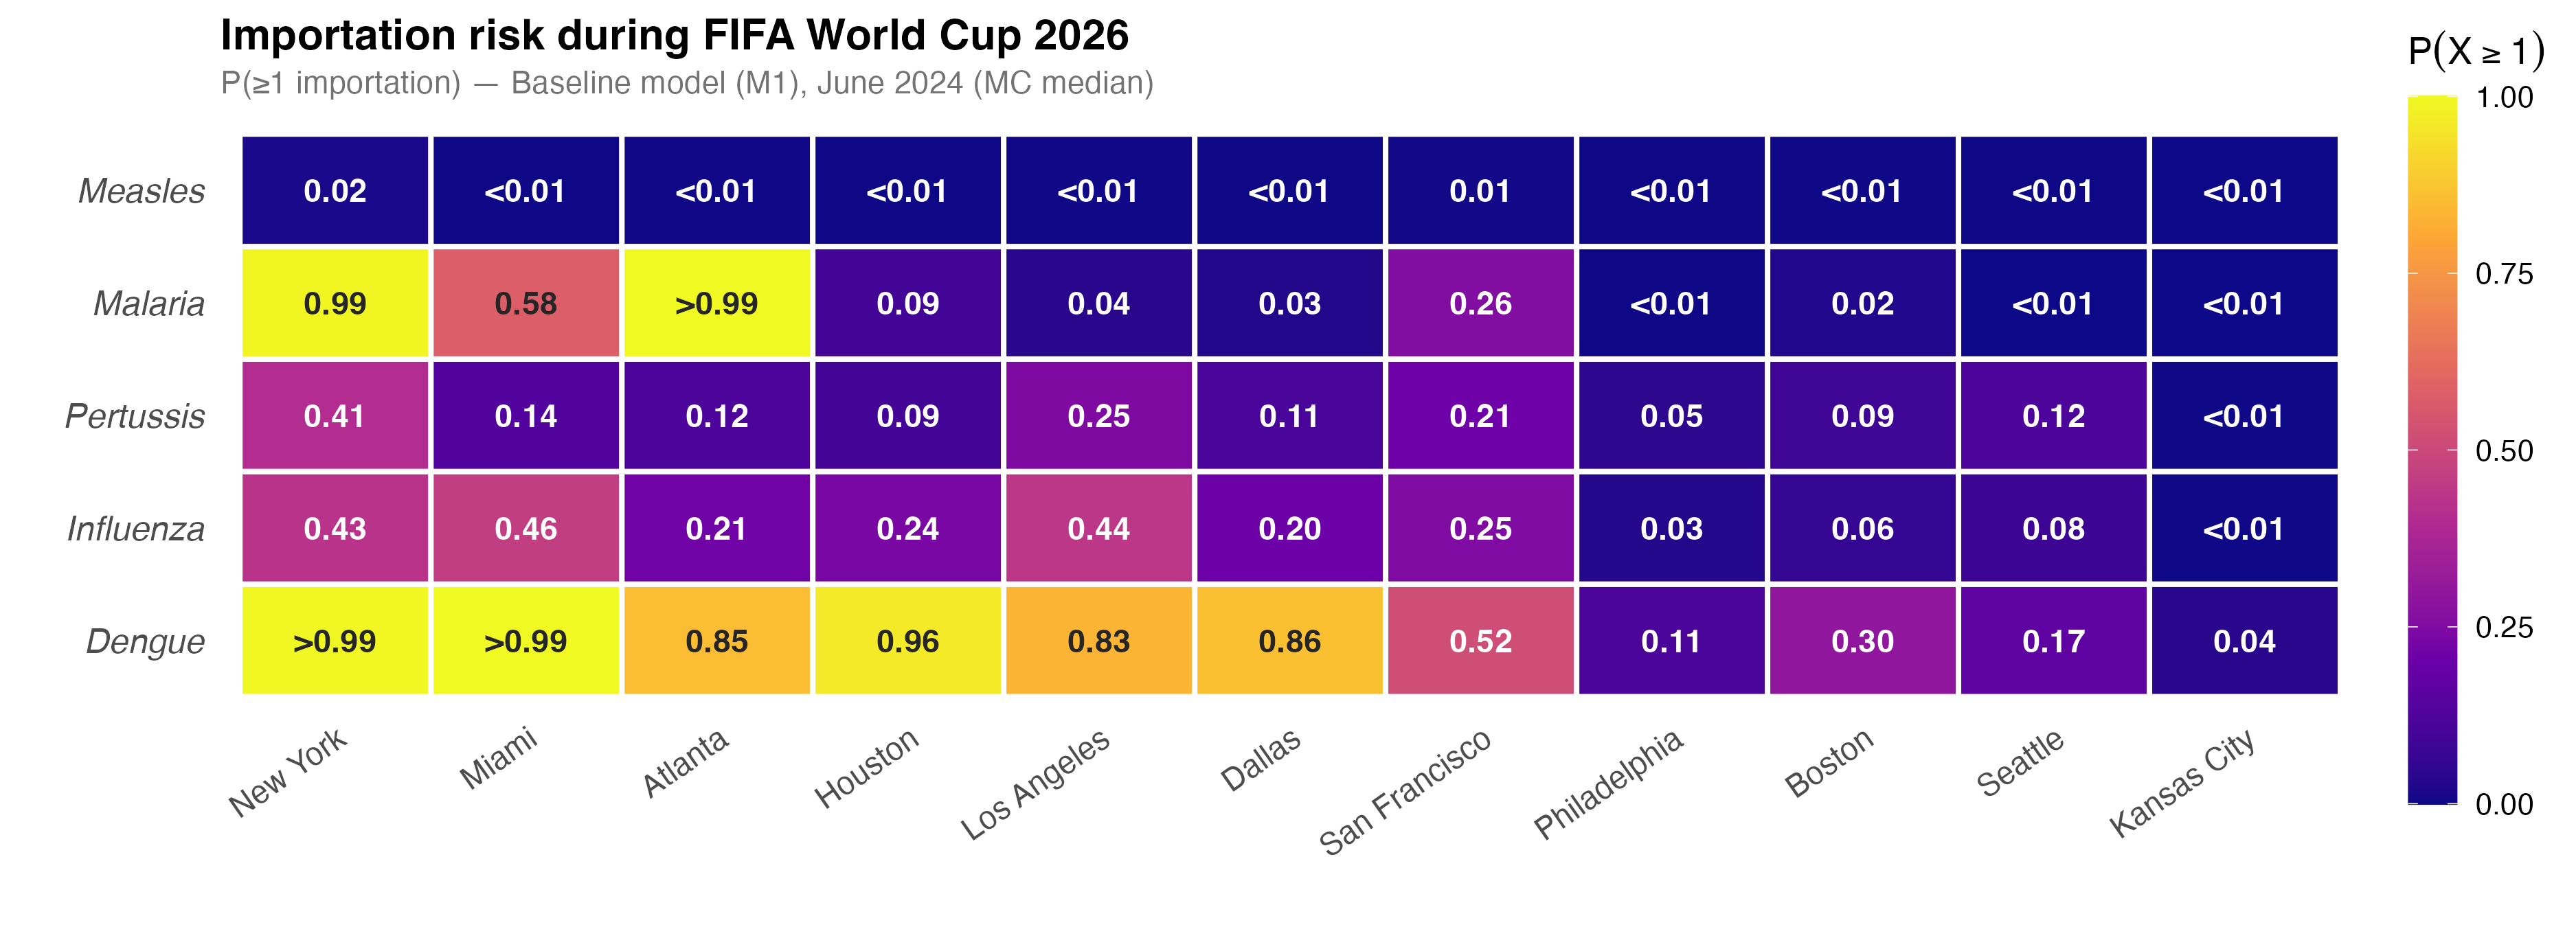
\includegraphics[width=\textwidth]{Figures/fig1_heatmap_baseline.png}
  \caption{Importation risk overview under the Baseline model (Model~1):
    $P(\geq 1\text{ importation})$ using routine June~2024 COR arrivals
    with no World Cup growth adjustment (MC median, 5,000 draws).
    Same city and disease ordering as Figure~1 in the main text.}
  \label{fig:heatmap_m1}
\end{figure}

\begin{figure}[h!]
  \centering
  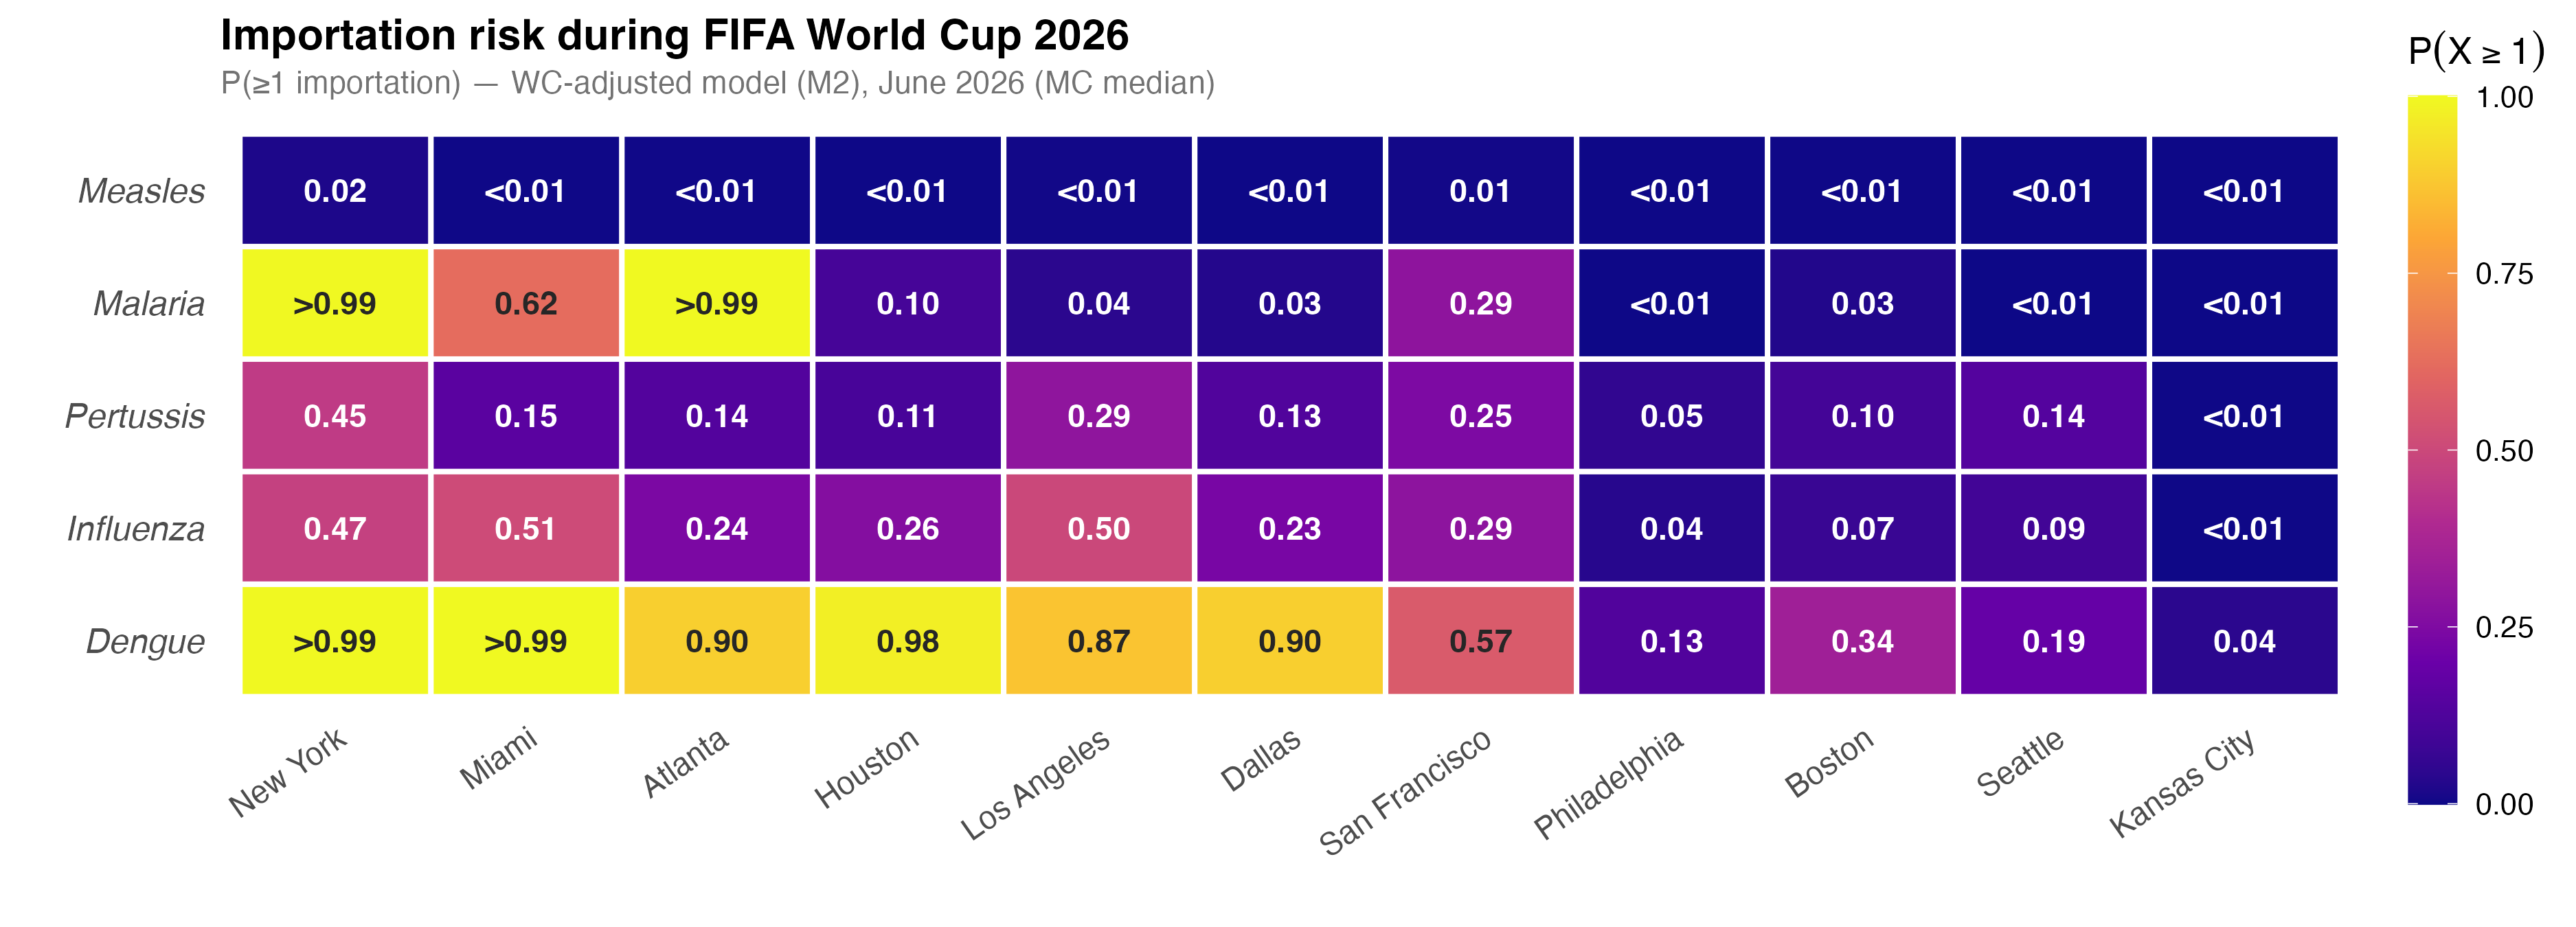
\includegraphics[width=\textwidth]{Figures/fig1_heatmap_wc.png}
  \caption{Importation risk overview under the WC-adjusted model (Model~2):
    $P(\geq 1\text{ importation})$ using June~2026 projected arrivals
    scaled by NTTO growth factors (MC median, 5,000 draws).
    Same city and disease ordering as Figure~1 in the main text.}
  \label{fig:heatmap_m2}
\end{figure}

\subsection*{Three-model comparison of importation intensity}

Figure~\ref{fig:model_comparison} compares expected importation intensity
($\Lambda$, median and 95\% MC uncertainty interval) across the three nested
model tiers for the six highest-risk US cities. The near-uniform step-up from
Model~1 to Model~2 reflects proportional amplification driven by the WC growth
factor; the further step to Model~3 introduces modest city-specific divergence
through schedule-based fan routing, without changing city or disease rankings.

\begin{figure}[h!]
  \centering
  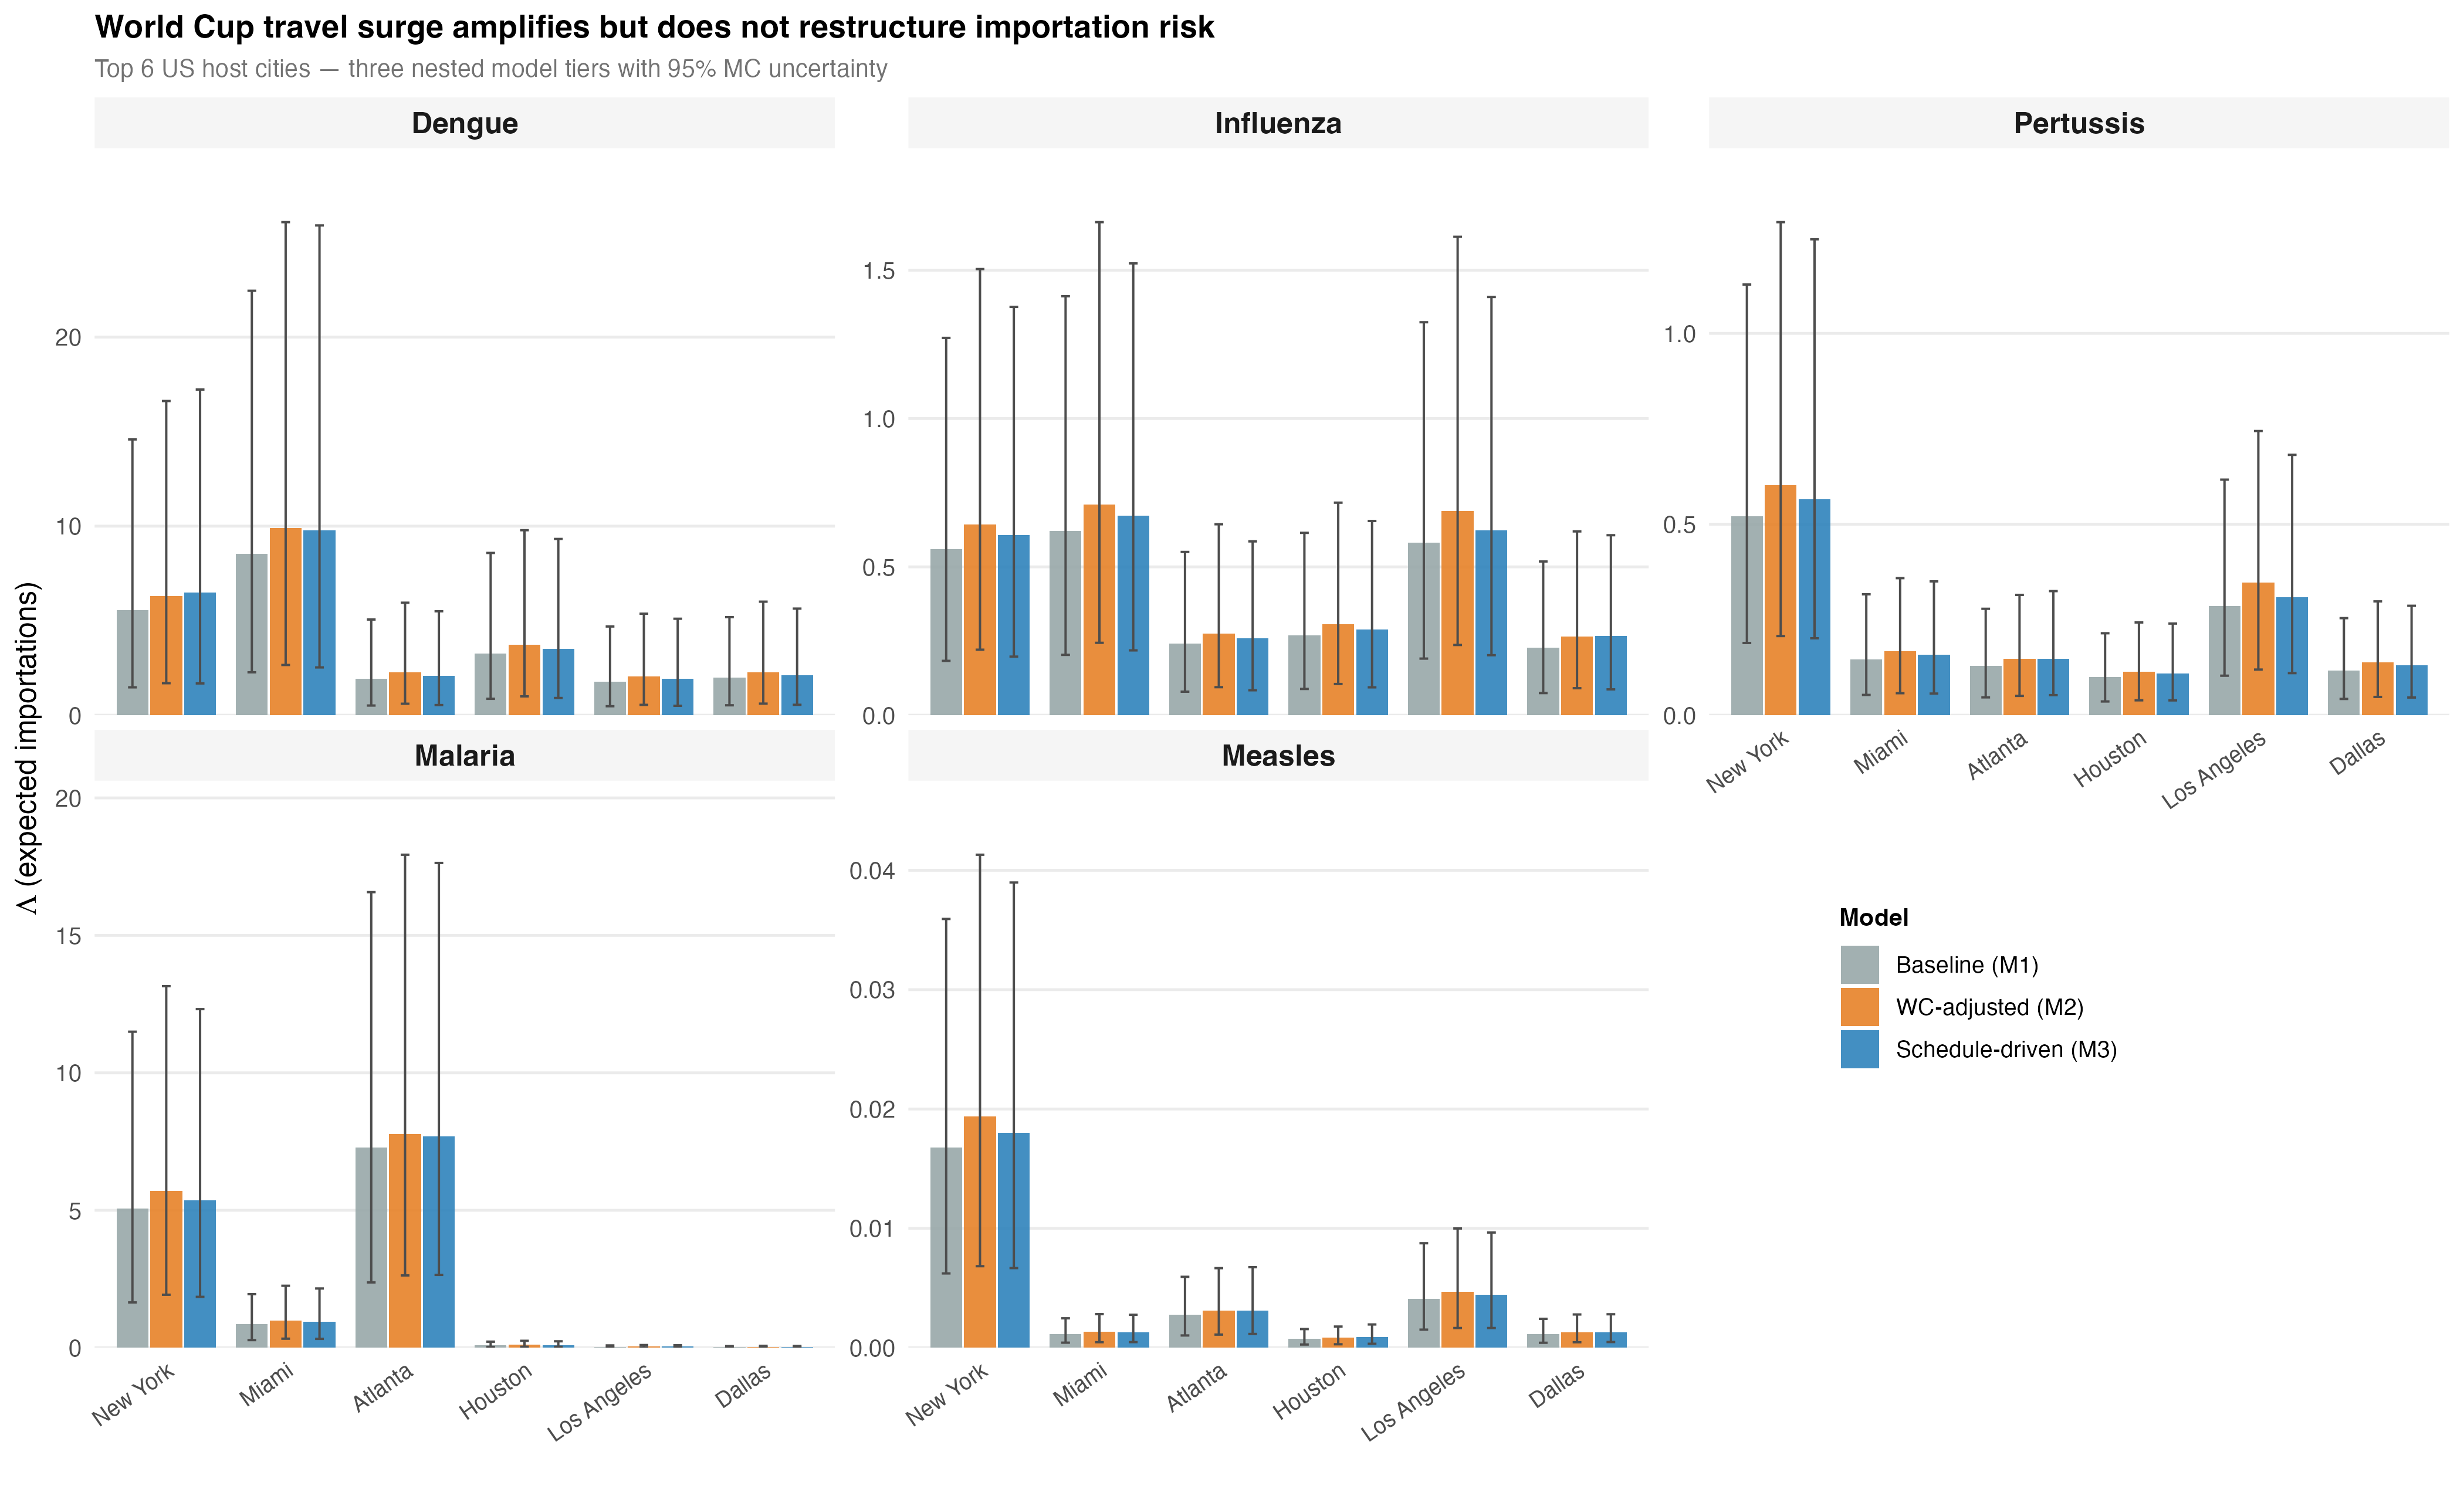
\includegraphics[width=\textwidth]{Figures/fig3_model_comparison.png}
  \caption{Three-model comparison of expected importations ($\Lambda$) for
    the six highest-risk US venue cities. Each panel shows one disease; bars
    are grouped by city and filled by model tier: Baseline (Model~1),
    WC-adjusted (Model~2), and Schedule-driven (Model~3). Bars show the MC
    median; whiskers span the 95\% uncertainty interval. The WC surge
    amplifies risk proportionally; schedule-based routing introduces modest
    city-specific divergence but leaves rankings unchanged.}
  \label{fig:model_comparison}
\end{figure}

\subsection*{Dengue stream decomposition by source country}

Figure~\ref{fig:stream_dengue} shows the dengue-specific travel
stream decomposition for the top~20 source countries: background
travel (blue) vs.\ WC fans (orange). The full five-disease stream
panel is Figure~\ref{fig:stream_panel}.

\begin{figure}[h!]
  \centering
  
\includegraphics[width=0.85\textwidth]{Figures/stream_breakdown_dengue.png}
  \caption{Dengue: importation intensity by travel stream for the
    top~20 source countries. Blue = background travel; orange = WC fans.
    Background dominates for all countries; the WC fan increment is
    largest for high-incidence WC-qualified nations
    (Brazil, Colombia, Ecuador).}
  \label{fig:stream_dengue}
\end{figure}

\subsection*{WC-fan vs.\ background travel stream decomposition}

Figure~\ref{fig:stream_panel} decomposes the top 20 contributing
countries by travel stream (WC fans vs.\ background) for each of
the five diseases. For WC-qualified countries, the WC-fan stream
contributes a meaningful but typically minority share of the total
importation intensity, consistent with the $\approx 8.3\%$ fan
fraction. Non-qualified countries contribute exclusively through the
background stream.

\begin{figure}[h!]
  \centering
  
\includegraphics[width=\textwidth]{Figures/stream_breakdown_panel.png}
  \caption{WC-fan vs.\ background travel stream decomposition for the
    top 20 source countries by total importation intensity, for each
    of the five diseases. \textcolor{orange!80!black}{Orange} = WC fans;
    \textcolor{blue!70!black}{Blue} = background. Countries with WC
    teams show a non-zero WC-fan component; non-qualified countries
    contribute only through background travel.}
  \label{fig:stream_panel}
\end{figure}

\subsection*{Country $\times$ city importation heatmaps}

Figures~\ref{fig:heatmap_dengue}--\ref{fig:heatmap_influenza} present
the country $\times$ city importation matrix ($\lambda_{c,v,d}$)
for each disease. WC-qualified countries from high-incidence regions
show importation concentrated at the venue cities where their team
plays, producing a block-diagonal structure aligned with the match
schedule. Non-qualified countries show importation spread diffusely
across cities in proportion to T-100 routing fractions.

\begin{figure}[h!]
  \centering
  
\includegraphics[width=\textwidth]{Figures/heatmap_dengue.png}
  \caption{Dengue importation matrix: expected importations
    $\lambda_{c,v}$ by source country (rows) and destination city
    (columns) under the schedule-driven model.}
  \label{fig:heatmap_dengue}
\end{figure}

\begin{figure}[h!]
  \centering
  
\includegraphics[width=\textwidth]{Figures/heatmap_malaria.png}
  \caption{Malaria importation matrix. Risk is concentrated in West
    and Central African source countries.}
  \label{fig:heatmap_malaria}
\end{figure}

\begin{figure}[h!]
  \centering
  
\includegraphics[width=\textwidth]{Figures/heatmap_measles.png}
  \caption{Measles importation matrix. Low absolute intensities
    across all cells reflect the low travel-while-infectious
    probability ($p = 0.05$).}
  \label{fig:heatmap_measles}
\end{figure}

\begin{figure}[h!]
  \centering
  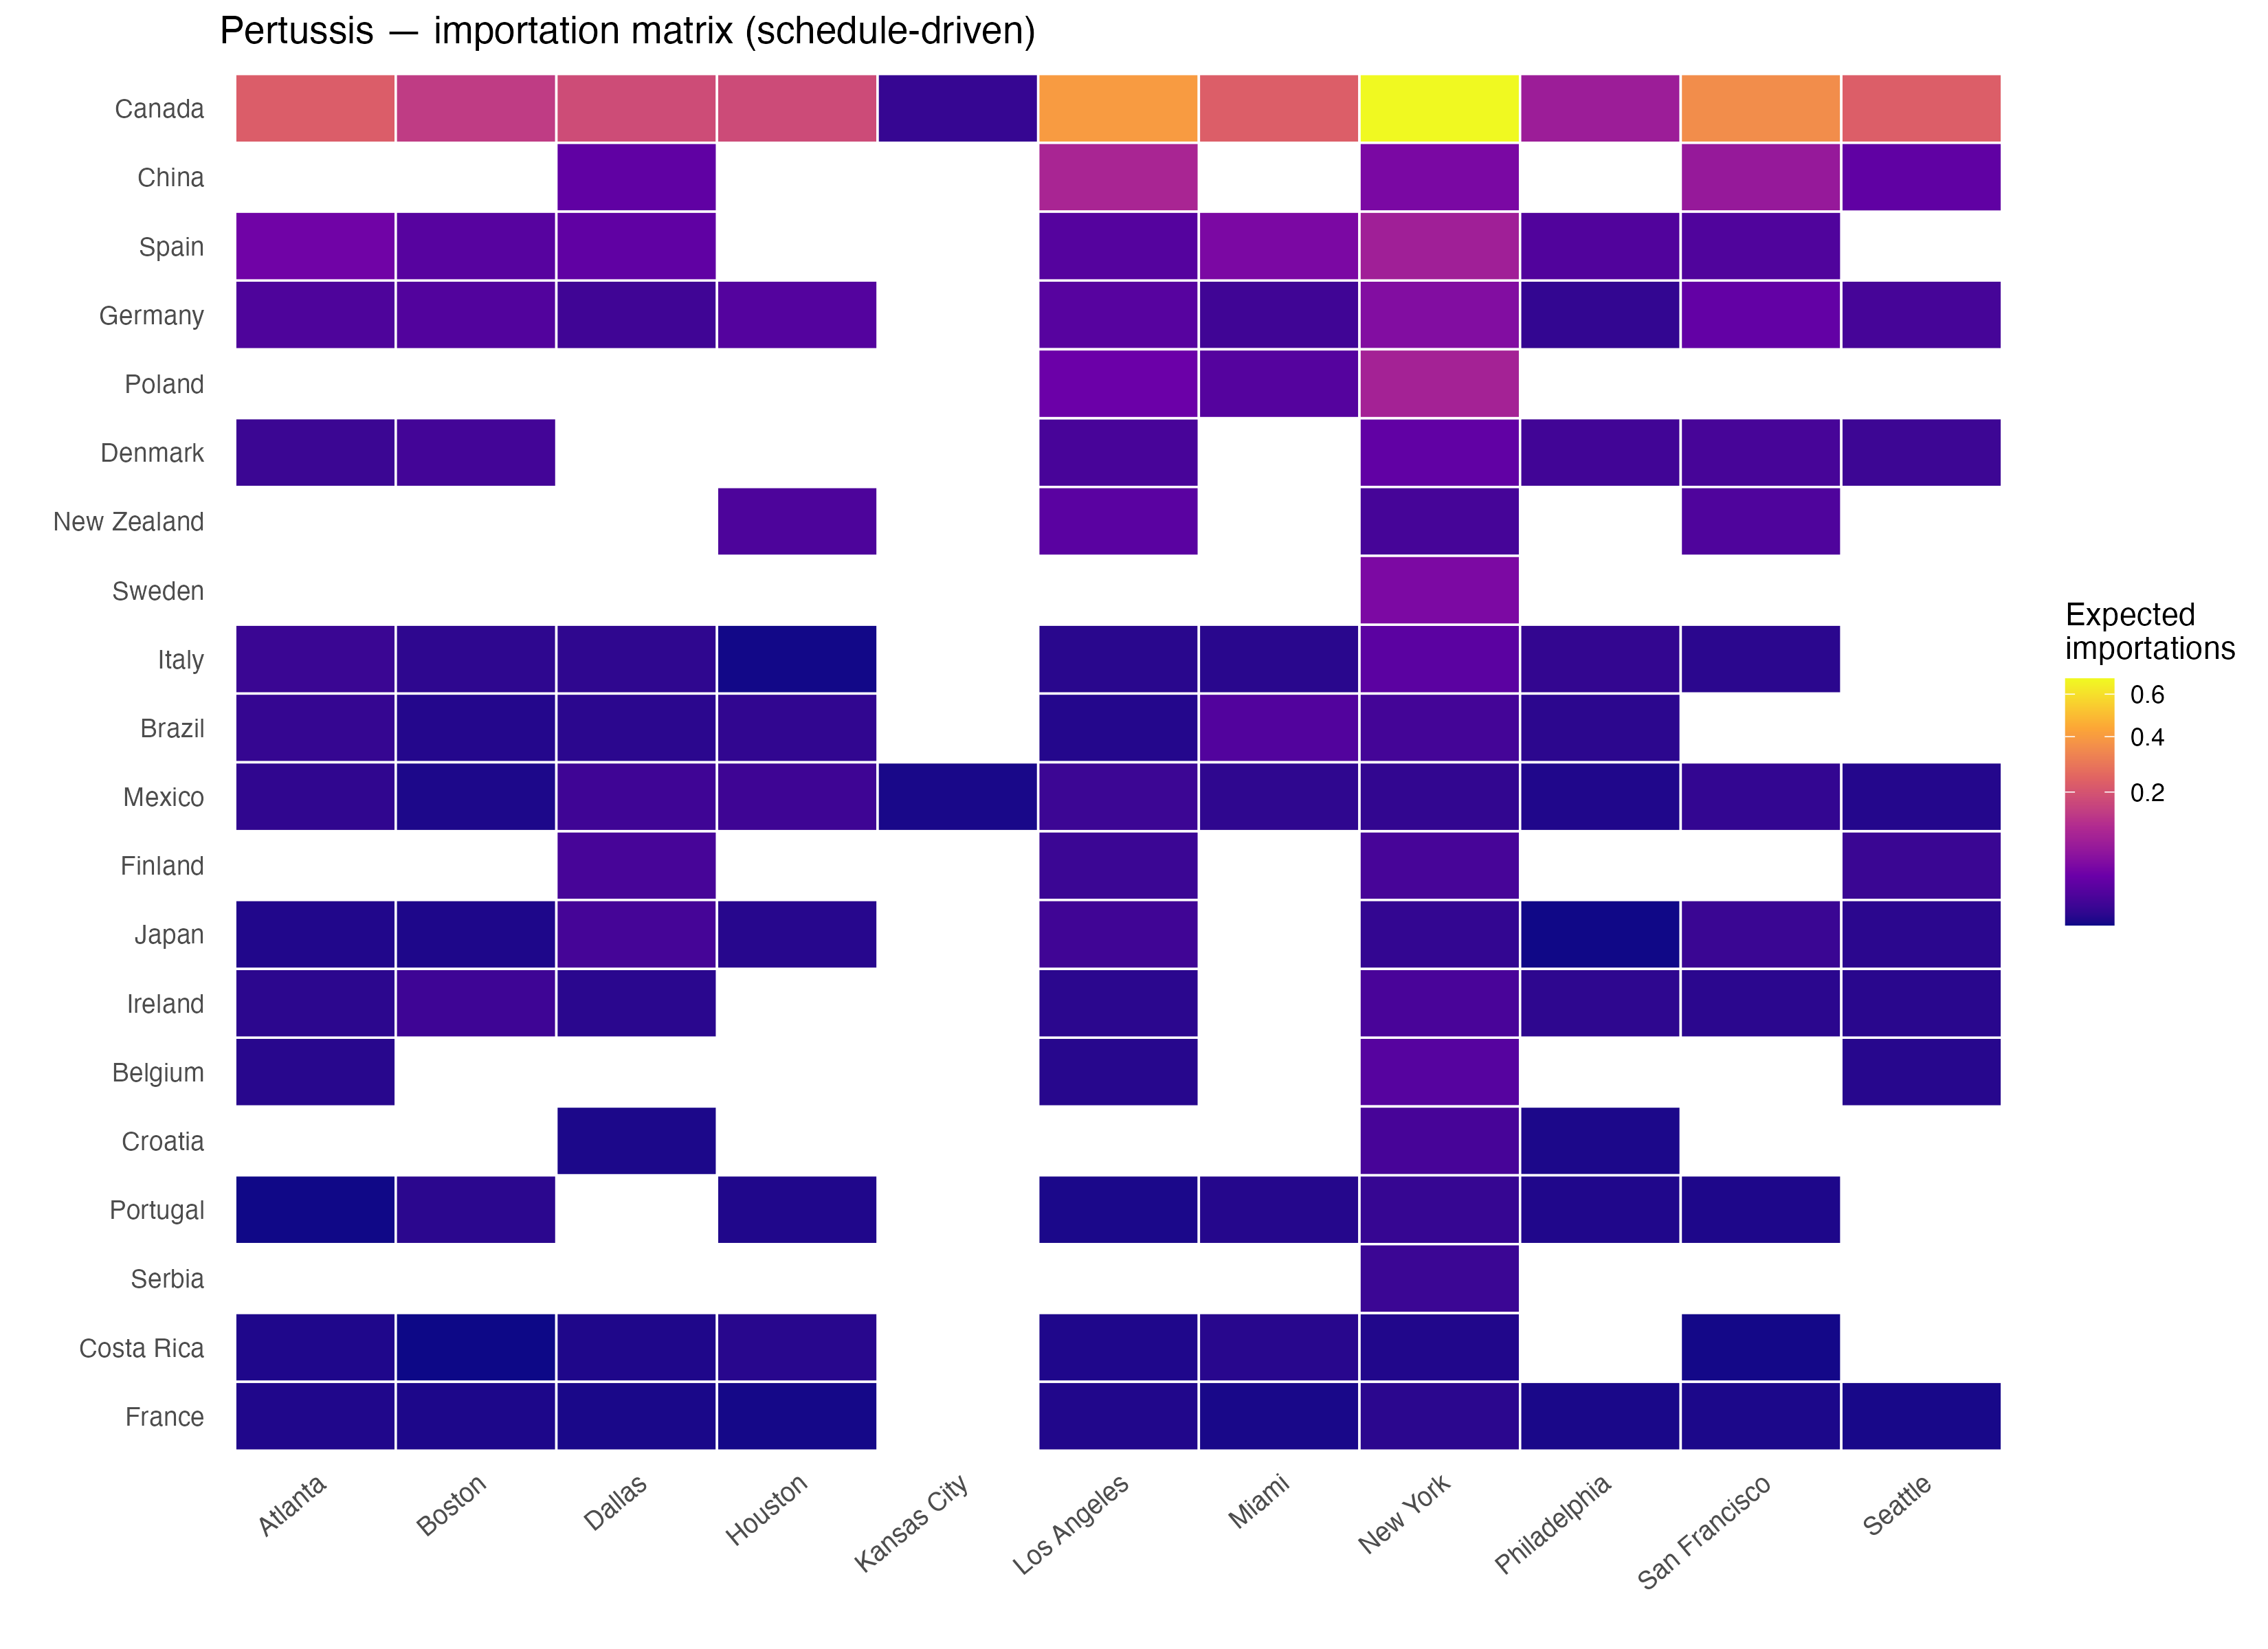
\includegraphics[width=\textwidth]{Figures/heatmap_pertussis.png}
  \caption{Pertussis importation matrix. The broad geographic spread
    reflects pertussis's global endemicity and high
    travel-while-infectious probability ($p = 0.70$).}
  \label{fig:heatmap_pertussis}
\end{figure}

\begin{figure}[h!]
  \centering
  
\includegraphics[width=\textwidth]{Figures/heatmap_influenza.png}
  \caption{Influenza importation matrix. Risk is highest for Southern
    Hemisphere nations (Brazil, Argentina, Colombia) whose June peak
    transmission coincides with the tournament window.}
  \label{fig:heatmap_influenza}
\end{figure}

% ============================================================
\section*{Appendix C: Data Limitations and Improvement Opportunities}
\addcontentsline{toc}{section}{Appendix C: Data Limitations and Improvement Opportunities}
% ============================================================

\subsection*{The role of non-public data in improving importation risk estimates}

The framework presented here relies entirely on publicly available
data sources --- a deliberate choice that ensures reproducibility and
allows the model to be updated by any public health team with internet
access. However, several categories of proprietary and restricted-access
data exist that would substantially improve the precision, timeliness,
and scope of the estimates, and their absence represents the primary
structural limitation of the current analysis.

The most valuable single dataset for this purpose would be
\textbf{airline booking and ticketing data}. Companies such as OAG
(Official Aviation Guide), Amadeus Travel Intelligence, and IATA's
PaxIS programme maintain origin-to-destination itinerary-level passenger
records that cover not only the nonstop international segment (as T-100
does) but the full trip, including domestic connecting legs to non-gateway
cities such as Kansas City and Seattle. These records are updated in
near-real time and can be filtered to the specific June--July 2026 travel
window rather than relying on historical routing fractions as a proxy for
future behavior. Similarly, \textbf{FIFA ticket sales records by country
of purchase}, while not publicly released, would replace the entire
WC-fan travel decomposition framework with a direct, event-specific
measure.

Beyond travel data, the precision of disease burden estimates is
constrained by the reliance on \textbf{WHO surveillance data}, which is
subject to reporting lags, inconsistent national case definitions, and
known under-ascertainment. National or regional health ministry
\textbf{line-list or case-count data} shared through WHO regional offices,
the Pan American Health Organization (PAHO), or the European Centre for
Disease Prevention and Control (ECDC) often contain more current and
complete figures than what appears in the publicly indexed datasets used
here. For measles and pertussis, \textbf{age-stratified incidence and
national vaccination coverage data} at the subnational level would
substantially improve the per-traveler infection probability $I_{c,d}$
by accounting for the fact that international travelers skew toward
working-age adults.

Finally, the current model estimates importation risk but stops short
of estimating local transmission risk after importation. Extending the
framework in that direction would require \textbf{local
\textit{Aedes aegypti} vector surveillance data} from state and
county health departments, \textbf{hospital and public health capacity
data} by city and county, and \textbf{aggregated mobility data} from
mobile device providers to calibrate the spatial spread of fans within
and between cities. Establishing data-sharing agreements with the
relevant agencies and commercial providers before the tournament
begins would allow these estimates to be refined and operationalized
in real time during June--July 2026.

% ============================================================
\newpage
\section*{Appendix D: Qualified Nations --- 2026 FIFA World Cup}
\addcontentsline{toc}{section}{Appendix D: Qualified Nations}
% ============================================================

\begin{longtable}{llc}
\toprule
\textbf{Country} & \textbf{Confederation} & \textbf{Host nation} \\
\midrule
\endfirsthead
\toprule
\textbf{Country} & \textbf{Confederation} & \textbf{Host nation} \\
\midrule
\endhead
\midrule
\multicolumn{3}{r}{\textit{Continued on next page}} \\
\endfoot
\bottomrule
\endlastfoot
% --- AFC (9) ---
Japan          & AFC & No \\
Iran           & AFC & No \\
South Korea    & AFC & No \\
Australia      & AFC & No \\
Qatar          & AFC & No \\
Saudi Arabia   & AFC & No \\
Uzbekistan     & AFC & No \\
Jordan         & AFC & No \\
Iraq           & AFC & No \\
% --- CAF (10) ---
Morocco        & CAF & No \\
Tunisia        & CAF & No \\
Egypt          & CAF & No \\
Algeria        & CAF & No \\
Ghana          & CAF & No \\
Cape Verde     & CAF & No \\
Senegal        & CAF & No \\
South Africa   & CAF & No \\
Ivory Coast    & CAF & No \\
DR Congo       & CAF & No \\
% --- CONCACAF (6) ---
Canada         & CONCACAF & Yes \\
Mexico         & CONCACAF & Yes \\
United States  & CONCACAF & Yes \\
Panama         & CONCACAF & No \\
Cura\c{c}ao   & CONCACAF & No \\
Haiti          & CONCACAF & No \\
% --- CONMEBOL (6) ---
Argentina      & CONMEBOL & No \\
Brazil         & CONMEBOL & No \\
Ecuador        & CONMEBOL & No \\
Paraguay       & CONMEBOL & No \\
Uruguay        & CONMEBOL & No \\
Colombia       & CONMEBOL & No \\
% --- UEFA (16) ---
England        & UEFA & No \\
France         & UEFA & No \\
Croatia        & UEFA & No \\
Portugal       & UEFA & No \\
Norway         & UEFA & No \\
Germany        & UEFA & No \\
Netherlands    & UEFA & No \\
Switzerland    & UEFA & No \\
Scotland       & UEFA & No \\
Spain          & UEFA & No \\
Austria        & UEFA & No \\
Belgium        & UEFA & No \\
Bosnia and Herzegovina & UEFA & No \\
Sweden         & UEFA & No \\
Turkey         & UEFA & No \\
Czech Republic & UEFA & No \\
% --- OFC (1) ---
New Zealand    & OFC & No \\
\end{longtable}

\noindent\small
\textit{Note}: Confederation abbreviations --- AFC: Asian Football
Confederation; CAF: Confederation of African Football; CONCACAF:
Confederation of North, Central America and Caribbean Association
Football; CONMEBOL: South American Football Confederation; UEFA:
Union of European Football Associations; OFC: Oceania Football
Confederation.

% ============================================================
\bibliographystyle{unsrtnat}
\bibliography{references}

\end{document}
